\documentclass[10pt,a4paper]{article}
\usepackage[latin1]{inputenc}
\usepackage{amsmath}
\usepackage{amsfonts}
\usepackage{amssymb}
\usepackage{makeidx}
\usepackage{graphicx}
\usepackage{caption}
\usepackage{subcaption}
\usepackage{float}
\usepackage{wrapfig}
\usepackage[left=1.00in, right=1.00in, top=1.00in, bottom=1.00in]{geometry}
\begin{document}
\title{TI Competition}
\author{Adam Leach, Edward Sainsbury, Kaiwen Lin, Oliver Groeling, Usmaan Javed}
\maketitle
\tableofcontents
\section{CAN Protocol}
\section{Driver Controls}
[INDICATORS AND BRAKE LIGHTS WIRING DIAGRAM]

[BLOCK DIAGRAM OF INDICATING/BRAKING(LIGHTS ONLY) PROCESS]

[EXPLAIN PICTURES DETAIL CONTROL MECHANISMS]

\section{Motor Communication}
[DIAGRAM SHOWING THE COMMUNICATION TO THE MOTOR CONTROLLER PROCESS]

[EXPLANATION OF DIAGRAM]

\section{Dashboard and Main Controller}
[PICTURE OF FINAL DASHBOARD]

[BRIEF DESCRIPTION OF HOW THE DRIVER CAN INTERFACE WITH IT]
The driver is able to interface with the dashboard / main controller through several switches. Firstly are the two switches which are wired to the dashboard; they can be used to configure what data is shown on the $7$ Segment Displays. For example, the left display could always show speed and the right display can toggle between battery level and temperature using the switches.

In addition to this there are two potentiometers which are connected to the break and acceleration pedals. The signal from this is converted into a digital signal using the ADC within the Launchpad. These signals are used to set the car's speed. There are also two more switches, one is ignition and the other is the directional indicator. 


[BLOCK DIAGRAM/SCHEMATIC OF MAIN CONTROLLER/DASHBOARD]
The schematic of the dashboard can be found in Figure \ref{fig:dashboard_schematic}. This board is to be directly connected to the main controller board, the schematic of which can be found [ADD MAINBOARD SCHEMATIC].
\begin{figure}%
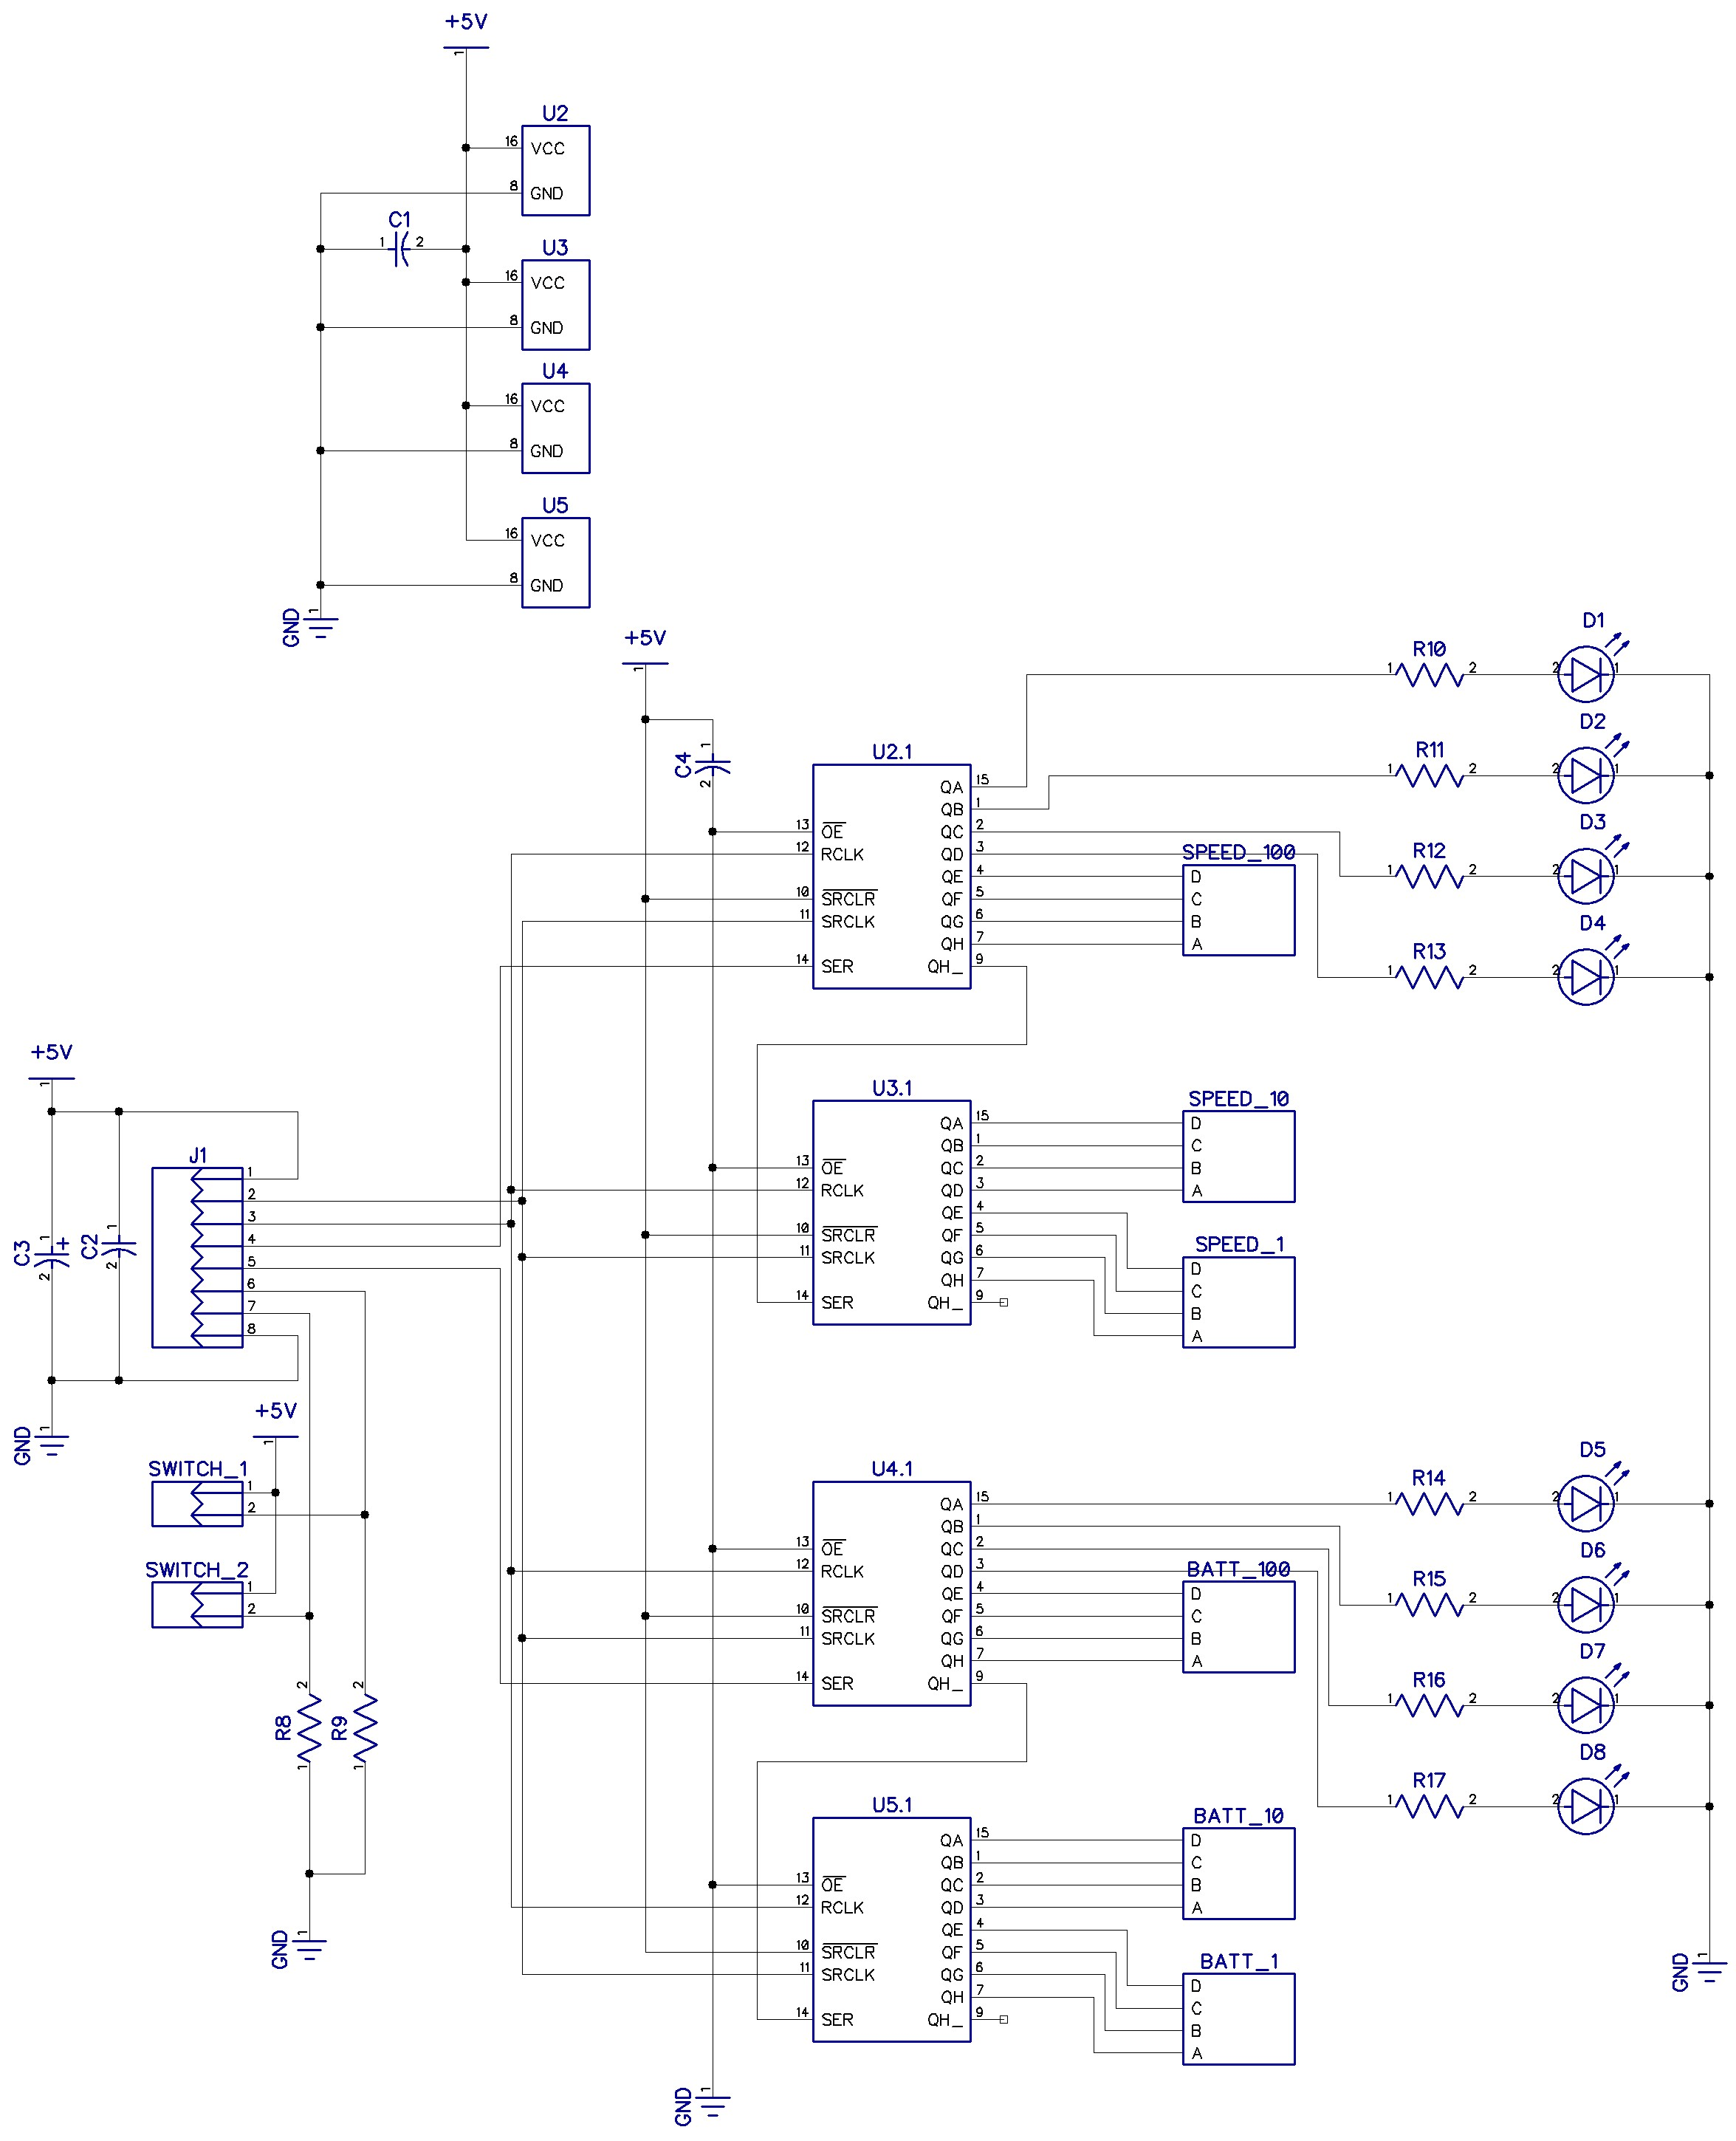
\includegraphics[width=\columnwidth]{dashboard_schematic.jpg}%
\caption{Dashboard Schematic}%
\label{fig:dashboard_schematic}%
\end{figure}

[EXPLANATION OF WHAT INPUTS THE MAIN CONTROLLER HANDLES AND WHAT OUTPUTS IT CONTROLS]

[EXPLANATION OF SAFETY FEATURES AND REDUNDANCIES BUILT INTO THE SYSTEM]

[VOLTAGE REGULATION INFO COULD GO HERE]

\section{Telemetry}
A crucial part of the project is the system that handles the large volume of data the CAN bus receives. This system must be able to efficiently store data, facilitate the sending of operation critical messages and provide meaningful feedback to the client.Telemetry is required to effectively analyze the system with both quantitative and qualitative data. This data will allow engineers to monitor the status of the system and make important decisions which could affect its performance. The proposed system can be broken down as follows: a CAN bus interface, a data logger, an SQL database, a graphical user interface to allow engineers to remotely access and send data.
\begin{wrapfigure}{r}{0.5\textwidth}
         \centering
         \begin{subfigure}[b]{0.6\textwidth}
                 \includegraphics[width=\textwidth]{canusb}
                 \caption{A CANUSB adaptor}
                 \label{fig:CANUSB adaptor}
         \end{subfigure}

         \begin{subfigure}[b]{0.4\textwidth}
                 \includegraphics[width=\textwidth]{beaglebone}
                 \caption{A Beagle Bone Black}
                 \label{fig:Beable Bone Black}
         \end{subfigure}

         \begin{subfigure}[b]{0.5\textwidth}
                 \includegraphics[width=\textwidth]{server}
                 \caption{A Server}
                 \label{fig:Sever}
         \end{subfigure}
         \caption{Components of the telemetry system}\label{fig:telemetry}
\end{wrapfigure}
The first component of the telemetry system is the interface between the data logger and the CAN bus. This connection is made with an adapter which connects directly in between the CANBUS and the data logger which is then controlled by the data handling software on the data logger.

The data is filtered by node and data type and is then saved to an SQL server running on the data logger. It is critically important that the data logger program can handle errors and consistently. If the program were to crash or incorrectly filter the data, the system could give incorrect data to the engineers leading to erroneous decisions or could completely stop working.

Once the data has been saved to the SQL server, the engineers can access or send data remotely over a tcp connection via a separate program on their computer. 

This is clearly a very powerful system allowing telemetry data to be sent and received from, theoretically,  anywhere in the world. If for example the nodes where in fact not just sensors but active components, it would be conceivable to drive the car from anywhere with an internet connection, thousands of miles away from the car itself.
\end{document}
